%%%%%%%%%%%%%%%%%%%%%%%%%%%%%%%%%%%%%%%%%%%%%%%%%%%%%%%%%%%%%%%%%%%%%%%%%%%%%%%%
%Tutorial slides on Python.
%
% Author: FOSSEE 
% Copyright (c) 2009, FOSSEE, IIT Bombay
%%%%%%%%%%%%%%%%%%%%%%%%%%%%%%%%%%%%%%%%%%%%%%%%%%%%%%%%%%%%%%%%%%%%%%%%%%%%%%%%

\documentclass[14pt,compress]{beamer}
%\documentclass[draft]{beamer}
%\documentclass[compress,handout]{beamer}
%\usepackage{pgfpages} 
%\pgfpagesuselayout{2 on 1}[a4paper,border shrink=5mm]

% Modified from: generic-ornate-15min-45min.de.tex
\mode<presentation>
{
  \usetheme{Warsaw}
  \useoutertheme{split}
  \setbeamercovered{transparent}
}

\usepackage[english]{babel}
\usepackage[latin1]{inputenc}
%\usepackage{times}
\usepackage[T1]{fontenc}

% Taken from Fernando's slides.
\usepackage{ae,aecompl}
\usepackage{mathpazo,courier,euler}
\usepackage[scaled=.95]{helvet}

\definecolor{darkgreen}{rgb}{0,0.5,0}

\usepackage{listings}
\lstset{language=Python,
    basicstyle=\ttfamily\bfseries,
    commentstyle=\color{red}\itshape,
  stringstyle=\color{darkgreen},
  showstringspaces=false,
  keywordstyle=\color{blue}\bfseries}

%%%%%%%%%%%%%%%%%%%%%%%%%%%%%%%%%%%%%%%%%%%%%%%%%%%%%%%%%%%%%%%%%%%%%%
% Macros
\setbeamercolor{emphbar}{bg=blue!20, fg=black}
\newcommand{\emphbar}[1]
{\begin{beamercolorbox}[rounded=true]{emphbar} 
      {#1}
 \end{beamercolorbox}
}
\newcounter{time}
\setcounter{time}{0}
\newcommand{\inctime}[1]{\addtocounter{time}{#1}{\tiny \thetime\ m}}

\newcommand{\typ}[1]{\lstinline{#1}}

\newcommand{\kwrd}[1]{ \texttt{\textbf{\color{blue}{#1}}}  }

%%% This is from Fernando's setup.
% \usepackage{color}
% \definecolor{orange}{cmyk}{0,0.4,0.8,0.2}
% % Use and configure listings package for nicely formatted code
% \usepackage{listings}
% \lstset{
%    language=Python,
%    basicstyle=\small\ttfamily,
%    commentstyle=\ttfamily\color{blue},
%    stringstyle=\ttfamily\color{orange},
%    showstringspaces=false,
%    breaklines=true,
%    postbreak = \space\dots
% }

%%%%%%%%%%%%%%%%%%%%%%%%%%%%%%%%%%%%%%%%%%%%%%%%%%%%%%%%%%%%%%%%%%%%%%
% Title page
\title[]{Interactive Plotting}

\author[FOSSEE] {FOSSEE}

\institute[IIT Bombay] {Department of Aerospace Engineering\\IIT Bombay}
\date[] {31, October 2009\\Day 1, Session 1}
%%%%%%%%%%%%%%%%%%%%%%%%%%%%%%%%%%%%%%%%%%%%%%%%%%%%%%%%%%%%%%%%%%%%%%

%\pgfdeclareimage[height=0.75cm]{iitmlogo}{iitmlogo}
%\logo{\pgfuseimage{iitmlogo}}


%% Delete this, if you do not want the table of contents to pop up at
%% the beginning of each subsection:
\AtBeginSubsection[]
{
  \begin{frame}<beamer>
    \frametitle{Outline}
    \tableofcontents[currentsection,currentsubsection]
  \end{frame}
}

\AtBeginSection[]
{
  \begin{frame}<beamer>
    \frametitle{Outline}
    \tableofcontents[currentsection,currentsubsection]
  \end{frame}
}

% If you wish to uncover everything in a step-wise fashion, uncomment
% the following command: 
%\beamerdefaultoverlayspecification{<+->}

%\includeonlyframes{current,current1,current2,current3,current4,current5,current6}

%%%%%%%%%%%%%%%%%%%%%%%%%%%%%%%%%%%%%%%%%%%%%%%%%%%%%%%%%%%%%%%%%%%%%%
% DOCUMENT STARTS
\begin{document}

\begin{frame}
  \maketitle
\end{frame}

%% \begin{frame}
%%   \frametitle{Outline}
%%   \tableofcontents
%%   % You might wish to add the option [pausesections]
%% \end{frame}


\begin{frame}[fragile]
\frametitle{Starting up...}
\begin{block}{}
\begin{verbatim}
  $ ipython -pylab  
\end{verbatim}
\end{block}
\begin{lstlisting}     
  In []: print "Hello, World!"
  Hello, World!
\end{lstlisting}
Exiting
\begin{lstlisting}     
  In []: ^D(Ctrl-D)
  Do you really want to exit([y]/n)? y
\end{lstlisting}
\end{frame}

\begin{frame}[fragile]
\frametitle{Loops}
Breaking out of loops
\begin{lstlisting}     
  In []: while True:
    ...:     print "Hello, World!"
    ...:     
  Hello, World!
  Hello, World!^C(Ctrl-C)
  ------------------------------------
  KeyboardInterrupt                   

\end{lstlisting}
\end{frame}

\begin{frame}[fragile]
\frametitle{First Plot}
\begin{columns}
    \column{0.25\textwidth}
    \hspace*{-0.5in}
  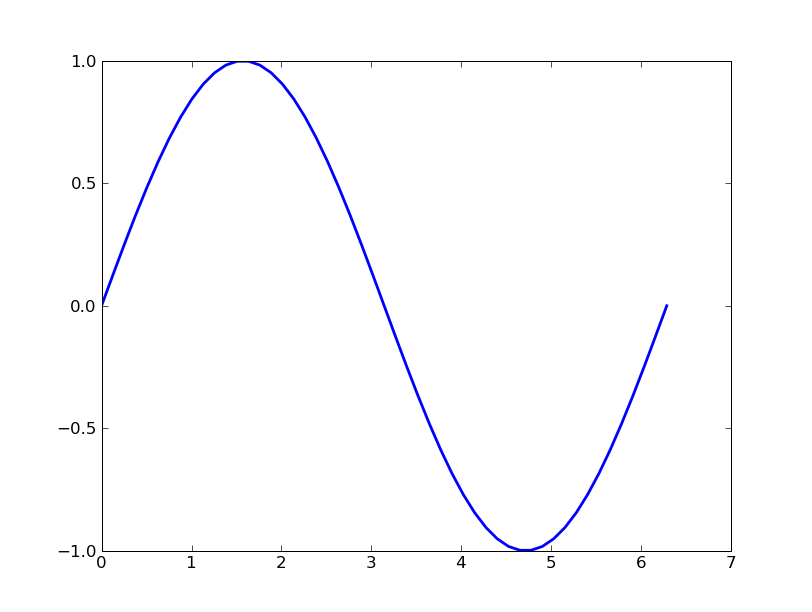
\includegraphics[height=2in, interpolate=true]{data/firstplot}  
    \column{0.8\textwidth}
    \begin{block}{}
    \small
\begin{lstlisting}
In []: x = linspace(0, 2*pi, 51)
In []: plot(x, sin(x))
\end{lstlisting}
    \small
    \end{block}
\end{columns}
\end{frame}


\begin{frame}[fragile]
\frametitle{Walkthrough}
\begin{block}{\typ{linspace(start, stop, num)} }
returns \typ{num} evenly spaced points, in the interval [\typ{start}, \typ{stop}].
\end{block}
\vspace*{.5in}
\begin{block}{\typ{plot(x, y)}}
plots \typ{x} and \typ{y} using default line style and color
\end{block}
\end{frame}

\begin{frame}[fragile]
\frametitle{Adding Labels}
\begin{columns}
  \column{0.25\textwidth}
  \hspace*{-0.45in}
  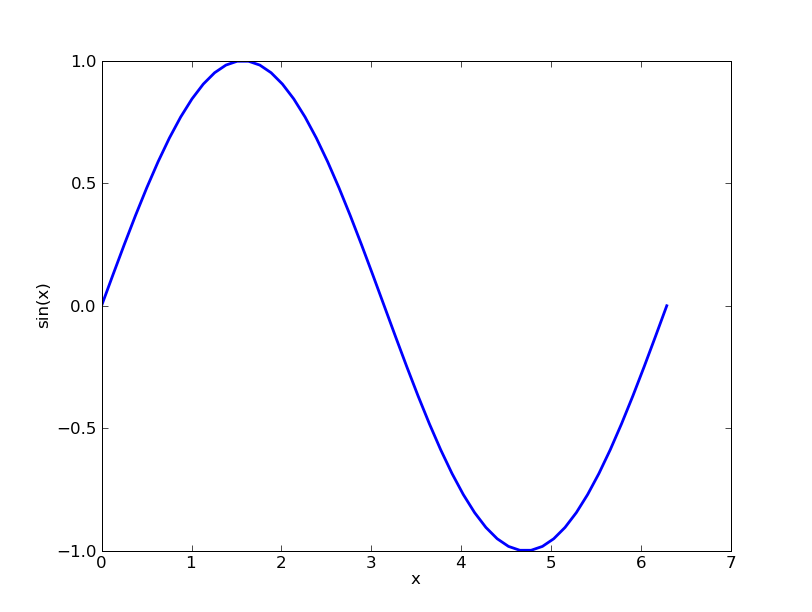
\includegraphics[height=2in, interpolate=true]{data/label}  
  \hspace*{0.5in}
  \column{0.55\textwidth}
  \begin{block}{}
  \small
  \begin{lstlisting}
In []: xlabel('x')

In []: ylabel('sin(x)')
  \end{lstlisting}
  \small
%  \end{lstlisting}
%\typ{xlabel(s)} sets the label of the \typ{x}-axis to \typ{s}

%  \begin{lstlisting}
  \end{block}
%\typ{ylabel(s)} sets the label of the \typ{y}-axis to \typ{s}
\end{columns}
\end{frame}

\begin{frame}[fragile]
\frametitle{Another example}
  \begin{lstlisting}
In []: clf()
In []: y = linspace(0, 2*pi, 51)
In []: plot(y, sin(2*y))
In []: xlabel('y')
In []: ylabel('sin(2y)')
  \end{lstlisting}
\end{frame}

\begin{frame}[fragile]
\frametitle{Title and Legends}
\vspace*{-0.15in}
%  \begin{block}{}
%  \small
\begin{lstlisting}
In []: title('Sinusoids')
#Sets the title of the figure
In []: legend(['sin(2y)'])
# When no label, or to change
\end{lstlisting}
%  \small
%  \end{block}
  \vspace*{-0.1in}
  \begin{center}
  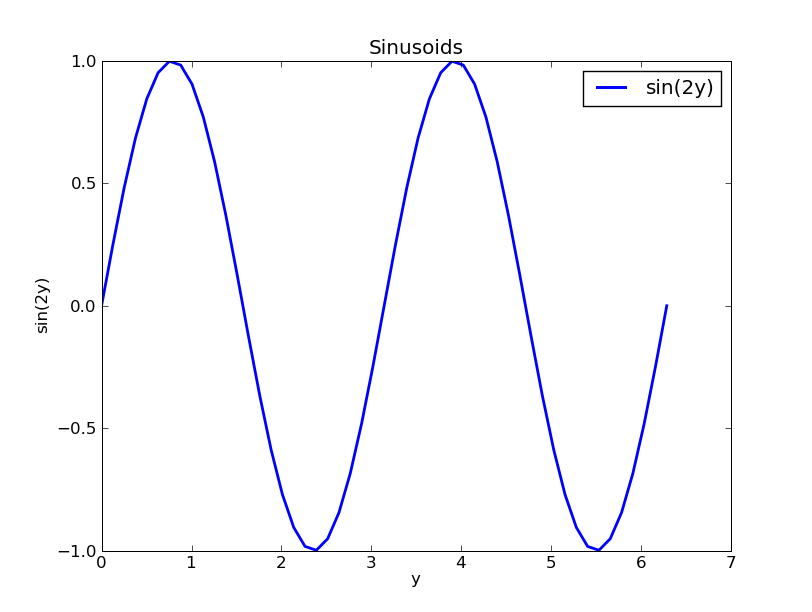
\includegraphics[height=2in, interpolate=true]{data/legend}  
  \end{center}
\end{frame}

\begin{frame}[fragile]
\frametitle{Changing Legend Placement}
\vspace*{-0.1in}
\begin{lstlisting}
In []: legend(['sin(2y)'], loc=(.8,.1)) 
#(x,y) is position of lower-left 
#corner of legend box.
\end{lstlisting}
%\vspace*{-0.2in}
\begin{center}
  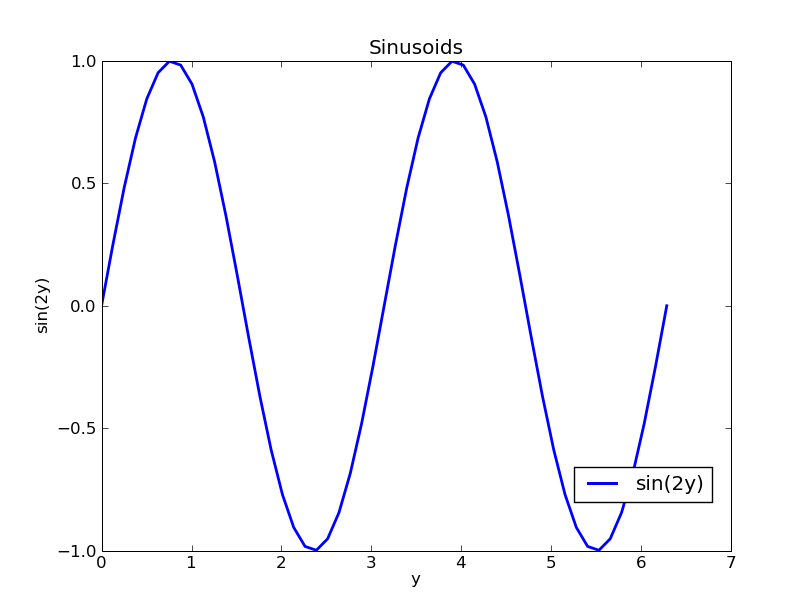
\includegraphics[height=2in, interpolate=true]{data/loc}  
\end{center}
\end{frame}

\begin{frame}[fragile]
\frametitle{Changing Legend Placement}
\begin{columns}
    \column{0.6\textwidth}
\begin{block}{}
    \small
\begin{lstlisting}
In []: legend(['sin(2y)'], 
         loc='right')
\end{lstlisting}
    \small
\end{block}
\column{0.45\textwidth}
\vspace{-0.2in}
\begin{lstlisting}
Location String   
===============   
'best'            
'upper right'     
'upper left'      
'lower left'      
'lower right'     
'right'           
'center left'     
'center right'    
'lower center'    
'upper center'    
'center'          
\end{lstlisting}
\end{columns}
\end{frame}


\begin{frame}[fragile]
\frametitle{Saving \& Closing}
\begin{lstlisting}
In []: savefig('sin.png')

In []: close()
\end{lstlisting}
\end{frame}

\begin{frame}[fragile]
\frametitle{Multiple Figures}
\begin{lstlisting}
In []: figure(1)
In []: plot(y, sin(y))
In []: figure(2)
In []: plot(y, cos(y))
In []: figure(1)
In []: title('sin(y)')
In []: close()
In []: close()
\end{lstlisting}
\end{frame}

\begin{frame}[fragile]
\frametitle{Showing it better}
\vspace{-0.15in}
\begin{lstlisting}
In []: plot(y, sin(y), 'g')

In []: clf()
In []: plot(y, sin(y), linewidth=2)
\end{lstlisting}
\vspace*{-0.2in}
\begin{center}
  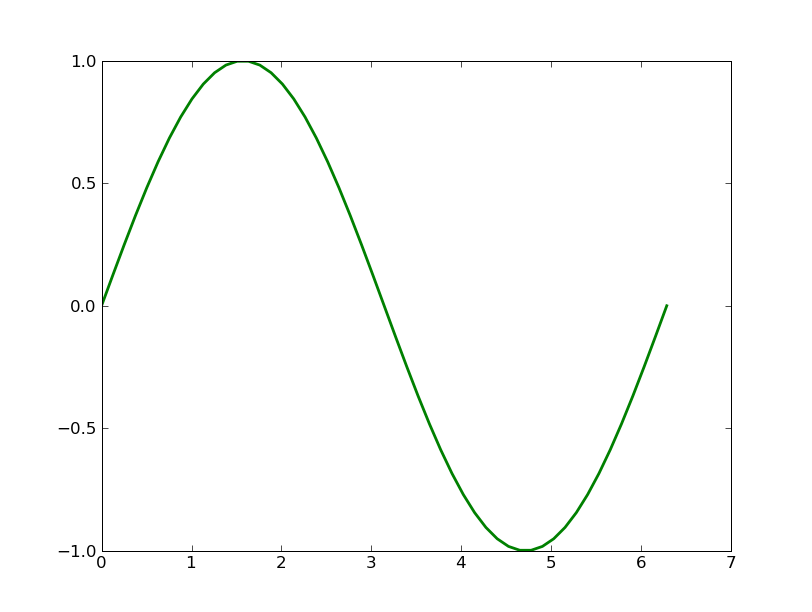
\includegraphics[height=2.2in, interpolate=true]{data/green}  
\end{center}
\end{frame}

\begin{frame}[fragile]
\frametitle{Annotating}
\vspace*{-0.15in}
\begin{lstlisting}
In []: annotate('local max', 
       xy=(1.5, 1), 
       xytext=(2.5, .8),
       arrowprops=dict(
       shrink=0.05),)
\end{lstlisting}
\vspace*{-0.2in}
\begin{center}
  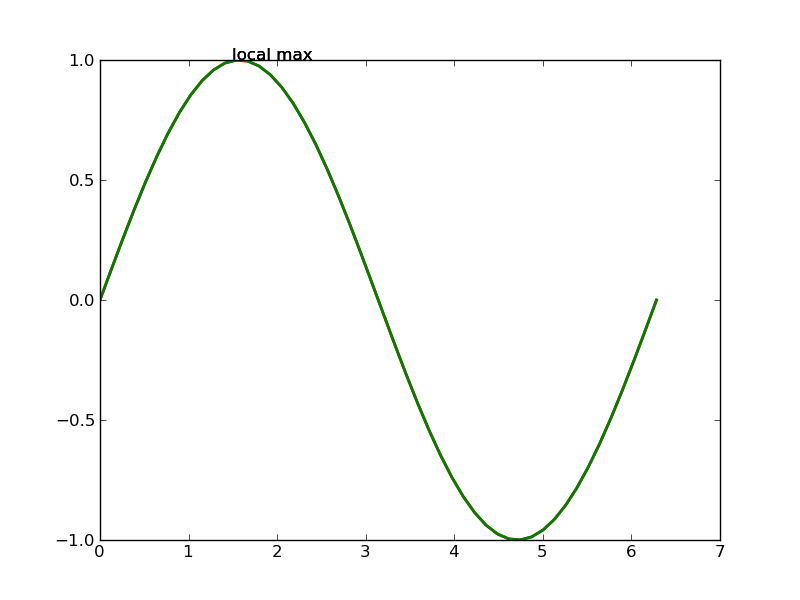
\includegraphics[height=2in, interpolate=true]{data/annotate}  
\end{center}
\end{frame}

\begin{frame}[fragile]
\frametitle{Axes lengths}
  \begin{lstlisting}
#Get the axes limits
In []: xmin, xmax = xlim() 
In []: ymin, ymax = ylim() 

In []: xmax = 2*pi
#Set the axes limits
In []: xlim(xmin, xmax) 
In []: ylim(ymin, ymax) 
  \end{lstlisting}
\end{frame}

\begin{frame}[fragile]
\frametitle{Review Problem}
\begin{enumerate}
\item Plot x, -x, sin(x), xsin(x) in the range $-5\pi$ to $5\pi$
\item Add a legend
\item Annotate the origin
\item Set axis limits to the range of x
\end{enumerate}
\begin{lstlisting}
In []: x=linspace(-5*pi, 5*pi, 501)
In []: plot(x, x, 'b')
In []: plot(x, -x, 'b')
\end{lstlisting}
$\vdots$
\end{frame}

\begin{frame}[fragile]
\frametitle{Review Problem \ldots}
\small{
\begin{lstlisting}
In []: plot(x, sin(x), 'g', linewidth=2)
In []: plot(x, x*sin(x), 'r', linewidth=3)
\end{lstlisting}

\begin{lstlisting}
In []: legend(['x', '-x', 'sin(x)', 'xsin(x)'])
In []: annotate('origin', 
                 xy=(0, 0), 
                 xytext=(0, -7),
                 arrowprops=dict(
                 shrink=0.05))
In []: xlim(5*pi, 5*pi)
In []: ylim(5*pi, 5*pi)
\end{lstlisting}
}
\end{frame}

\begin{frame}[fragile]
  \begin{center}
  End of Session-1\\
  \alert{Don't Close \typ{IPython}}
  \end{center}
\end{frame}

\end{document}

